%%%%%%%%%%%%%%%%%%%%%%%%%%%%%%%%%%%%%%%%%
% Stylish Article
% LaTeX Template
% Version 2.1 (1/10/15)
%
% This template has been downloaded from:
% http://www.LaTeXTemplates.com
%
% Original author:
% Mathias Legrand (legrand.mathias@gmail.com) 
% With extensive modifications by:
% Vel (vel@latextemplates.com)
%
% License:
% CC BY-NC-SA 3.0 (http://creativecommons.org/licenses/by-nc-sa/3.0/)
%
%%%%%%%%%%%%%%%%%%%%%%%%%%%%%%%%%%%%%%%%%

%----------------------------------------------------------------------------------------
%	PACKAGES AND OTHER DOCUMENT CONFIGURATIONS
%----------------------------------------------------------------------------------------

\documentclass[fleqn,11pt]{SelfArx} % Document font size and equations flushed left

\usepackage[ngerman]{babel} % Specify a different language here - english by default

\usepackage{eurosym}
\usepackage[utf8]{inputenc}
\DeclareUnicodeCharacter{20AC}{\euro}

\usepackage{tocloft}

\usepackage{lipsum} % Required to insert dummy text. To be removed otherwise

\usepackage{csquotes}

\usepackage{float}

%----------------------------------------------------------------------------------------
%	COLUMNS
%----------------------------------------------------------------------------------------

\setlength{\columnsep}{0.55cm} % Distance between the two columns of text
\setlength{\fboxrule}{0.75pt} % Width of the border around the abstract
\setlength{\cftfignumwidth}{2.55em}

%----------------------------------------------------------------------------------------
%	COLORS
%----------------------------------------------------------------------------------------

\definecolor{color1}{RGB}{0,0,0} % Color of the article title and sections
\definecolor{color2}{RGB}{40,180,220} % Color of the boxes behind the abstract and headings
\def \boxTransparency {20} % Percentage of transparency

%----------------------------------------------------------------------------------------
%	HYPERLINKS
%----------------------------------------------------------------------------------------

\usepackage{hyperref} % Required for hyperlinks
\hypersetup{hidelinks,colorlinks,breaklinks=true,urlcolor=color2,citecolor=color1,linkcolor=color1,bookmarksopen=false,pdftitle={Title},pdfauthor={Author}}

%----------------------------------------------------------------------------------------
%	TABLES
%----------------------------------------------------------------------------------------

\usepackage[normalem]{ulem}
\useunder{\uline}{\ul}{}

%----------------------------------------------------------------------------------------
%	ARTICLE INFORMATION
%----------------------------------------------------------------------------------------


\Fach{Mobile Anwendungen mit Android}
\Semester{Sommersemester 2018}
\Abgabedatum{06.07.2018}

\PaperTitle{BOSCall - Dokumentation} % Article title

\Authors{Dorian Weidler, B.Sc. (868407) - Christoph Suffel, B.Sc. (866555)} % Authors
\affiliation{\textbf{Corresponding authors}: dowe0012@stud.hs-kl.de, chsu0001@stud.hs-kl.de} % Corresponding author

\Keywords{Android --- Feuerwehr --- Alarmierung} % Keywords - if you don't want any simply remove all the text between the curly brackets
\newcommand{\keywordname}{Keywords} % Defines the keywords heading name

%----------------------------------------------------------------------------------------
%	ABSTRACT
%----------------------------------------------------------------------------------------

\Abstract{BOSCall wurde im Rahmen der Veranstaltung Mobile Anwendungen mit Android an der Hochschule Kaiserslautern im Sommersemester 2018 entwickelt. Der betreuende Dozent der Arbeit war Prof. Dr. Manh Tien Tran.
	
	Ziel der Veranstaltung war die Entwicklung einer Android App. Die Entscheidung fiel recht schnell, dass eine App zur mobilen Alarmierung von Einsatzkräften entwickelt werden sollte. Zum Zeitpunkt der Entwicklung gab es keine kostengünstige beziehungsweise kostenlose Variante für mehrheitlich ehrenamtlich besetzte Behörden mit Sicherheitsaufgaben (BOS).
	BOSCall soll als Open-Source Ansatz jeder Feuerwehr mit dem nötigen Know-How eine Basis geben Ihre Einsatzkräfte zusätzlich auch über ihr privates mobiles Endgerät zu alarmieren. Durch die hohe Verbreitung von Smartphones und die stetig flächendeckendere Mobilfunkabdeckung kann durch diesen Zusatzalarmiert mit einer hohen Wahrscheinlichkeit der Alarm jedes einzelnen Mitglieds sichergestellt werden.}

%----------------------------------------------------------------------------------------

\hypersetup{draft}
\begin{document}

\flushbottom % Makes all text pages the same height

\maketitle % Print the title and abstract box

\tableofcontents % Print the contents section

\thispagestyle{empty} % Removes page numbering from the first page

%----------------------------------------------------------------------------------------
%	ARTICLE CONTENTS
%----------------------------------------------------------------------------------------

\section{Einleitung}
Für Fördervereine der freiwilligen Feuerwehr ist es eine massive Kostenbelastung, wenn bereits wenige hundert Euro jedes Jahr zu bezahlen sind. Die Träger der Feuerwehren berufen sich bezüglich der Alarmierung per Smartphone darauf, dass bereits durch analoge oder digitale Meldeempfänger ausreichend vorgesorgt ist und die Einsatzkräfte adäquat alarmiert werden.

In der Feuerwehr Kusel wurde beispielsweise eine\\ firEmergency\cite{Alamos:FE2} Installation betrieben, die durch den Förderverein finanziert wurde. Das heißt Spenden, Mitgliederbeiträge und Veranstaltungserlöse werden genutzt um eine grundlegende Anforderung sicherzustellen. Ein Kostenvergleich zwischen einer aktuellen {firEmergency 2} Installation und der BOSCall Variante folgt in Kapitel~\ref{sec:kostenvergleich}.

\section{Kostenvergleich}
\label{sec:kostenvergleich}
Wie bereits einleitend erwähnt und auch technisch bedingt entstehen Kosten, um diese Art von digitalem Alarm zu realisieren. Zunächst soll hierbei auf eine fertige Lösung von einem etablierten Anbieter eingegangen werden. Diese ist bereits in der Feuerwehr Kusel, die als Testeinheit dient, in einer älteren, nicht mehr verfügbaren Version im Einsatz. Die App nennt sich APager (Pro), die Backend Software, die unabdingbar für die App ist, nennt sich firEmergency. Beides sind fertige Lösungen der Firma Alamos GmbH.

Betrachtet wird im Folgenden eine Lösung auf Basis einer serverseitigen Lizensierung. Das heißt die Kosten fallen auf Seiten des Betreibers an und sind entsprechend in Summe günstiger als der Kauf einzelner Lizenzen pro App. Die Preise stammen von \cite{Alamos:FE2Pricing}. Unterstützt werden soll eine Nutzerbasis von 200 Personen.
\begin{table}[]
	\centering
	\caption{Kostenaufstellung APager \& firEmergency}
	\label{tbl:FE2Pricing}
	\begin{tabular}{|l|r|}
		\hline
		{\ul \textbf{Beschreibung}}        & \multicolumn{1}{l|}{{\ul \textbf{Preis}}} \\ \hline
		firEmergency Paket 1 (30 Personen) & 179,99 €/Jahr                             \\ \hline
		+170 Personen                      & 593,30 €/Jahr                             \\ \hline
		Windows Office PC                  & ca. 400€                                  \\ \hline
	\end{tabular}
\end{table}

Bei der Aufstellung der Kosten in Tabelle~\ref{tbl:FE2Pricing} wurde berücksichtigt, dass Einzelpersonen günstiger sind als die größeren Pakete, wenn man wirklich nur die Personen und nicht weitere Features benötigt. Da BOSCall die anderen Features nicht bietet wird der Fairness halber mit dem preislich günstigsten Paket und den zusätzlichen Personen gerechnet. Ein Computer mit Windows Betriebssystem ist erforderlich um firEmergency zu betreiben.\cite{Alamos:FE2SystemRequirements} Aufsummiert fallen im ersten Jahr bereits 1173,29~€ an. In den Folgejahren, unter der Vorraussetzung die Preise ändern sich nicht und der Rechner wird einfach stetig weiterbetrieben, 773,29~€.

Das ist für einen kleinen, gemeinnützigen Verein kaum zu stemmen, insbesondere weil es sich nicht um einmalige sondern laufende Kosten handelt. Die Ersatz"-lösung, die im Rahmen dieser Veranstaltung entwickelt wurde, soll diese Kosten also drastisch unterschreiten, damit sich der zusätzliche Aufwand rechtfertigt. In Tabelle~\ref{tbl:BOSCallPricing} befindet sich eine Beispielaufstellung der Kosten, mit denen zu rechnen ist, um BOSCall zu betreiben. Da die Anwendung noch nicht in der Praxis erprobt ist, handelt es sich dabei zunächst um eine rein theoretische Aufstellung sämtlicher Kosten.

\begin{table}[]
	\centering
	\caption{Kostenaufstellung BOSCall}
	\label{tbl:BOSCallPricing}
	\begin{tabular}{|l|r|}
		\hline
		{\ul \textbf{Beschreibung}} & \multicolumn{1}{l|}{{\ul \textbf{Preis}}} \\ \hline
		Google Entwickler Zugang    & \$ 25                                     \\ \hline
		Virtueller Server           & 5 €/Monat                                 \\ \hline
		Raspberry Pi m. Zubehör     & 50 €                                      \\ \hline
		USB Soundkarte              & 6,25 €                                    \\ \hline
	\end{tabular}
\end{table}

Man erkennt direkt, dass die Kosten erheblich geringer sind. Zudem verteilen sie sich fast nur auf einmalige Kosten. Der Google Entwickler Zugang ist erforderlich um Apps im Play Store zu veröffentlichen und sie so der breiten Masse an Feuerwehrmitgliedern der Feuerwehr Kusel einfach zugänglich zu machen. Der virtuelle Server ist für das Bereitstellen der Backend API erforderlich. Was der Dienst können muss wird in Kapitel~\ref{sec:funktionsweise} erläutert.  Der Raspberry Pi mit der USB Soundkarte ist für die lokale Installation eines Alarmauswerters erforderlich. Auch dabei wieder der Verweis auf Kapitel~\ref{sec:funktionsweise}. In Summe liegt man dabei im ersten Jahr bei ca. 137,75 €, abhängig vom Wechselkurs des Dollar. In den Folgejahren belaufen sich die Kosten auf 60 €. Dabei besteht zusätzlich der große Vorteil, dass man auch problemlos mehr Mitglieder anlegen kann ohne, dass sich die jährlichen Kosten erhöhen. Bereits der schwächste Linux Server, der heute üblicherweise angeboten wird, bietet erheblich mehr Leistung als erforderlich.

\section{Funktionsweise}
\label{sec:funktionsweise}
Prinzipiell dreht sich die App um zwei essentielle Funktionen. Die Registration und der Alarmempfang. Diese beiden Funktionalitäten werden nachfolgend genauer beschrieben.
\subsection{Registration}
\begin{figure}[htbp]
	\centering
	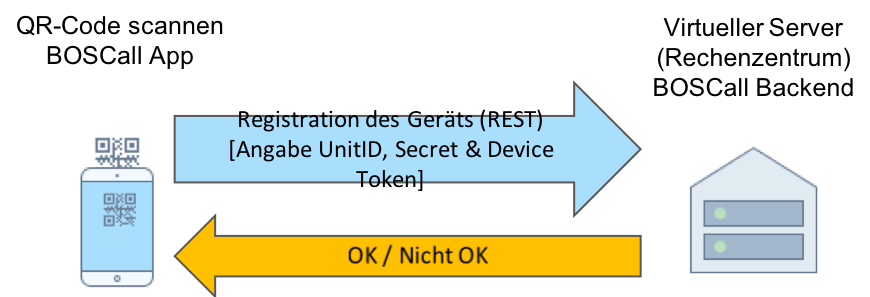
\includegraphics[width=\linewidth]{include/img/registration}
	\caption{Registration}
	\label{fig:registration}
\end{figure}
Anforderungen an die Registration war eine möglichst geringe Komplexität und zugleich eine hohe Sicherheit zu realisieren. Der Fokus lag aber zwecks des begrenzten Entwicklungszeitraums auf der geringen Komplexität.

Um die Komplexität zu reduzieren wird jedem Leiter einer Einheit ein QR-Code ausgestellt, der dazu dient, dass sich Mitglieder registrieren können. Es ist für den Anwender also nur erforderlich, dass er seinen Namen eingibt und einen QR-Code mit seiner Smartphone Kamera scannt. In diesem QR-Code befinden sich alle Details, die zur Registration erforderlich sind. Zum Beispiel die ID der Einheit (UnitID) und der private Schlüssel (Secret). Zusätzlich sendet das Gerät bei der Registrationsanfrage den eigenen Gerätetoken (Devicetoken) mit. Damit können Push Nachrichten gezielt an das Endgerät gesendet werden.

\subsection{Alarmempfang}
\begin{figure*}[htbp]
	\centering
	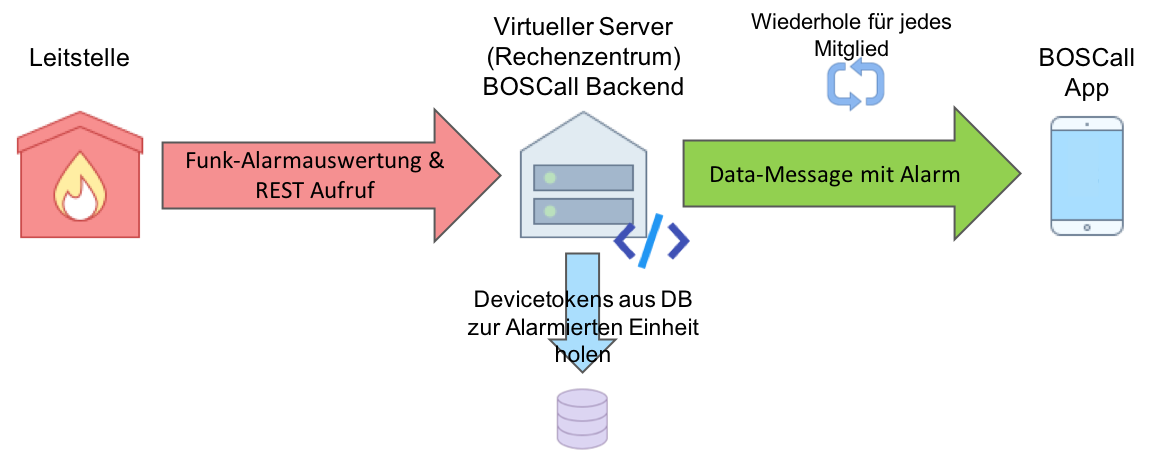
\includegraphics[width=\linewidth]{include/img/alarmablauf}
	\caption{Alarmablauf}
	\label{fig:alarmablauf}
\end{figure*}
Der Ablauf der Alarmierung, graphisch in Abbildung~\ref{fig:alarmablauf} zu sehen, teilt sich in drei Schritte. Zunächst wird der Alarm über eine Auswertung des analogen Funks erkannt und es wird die E-Mail der Leitstelle mit den Einsatzdetails ausgewertet. Dieser Prozess wird nicht durch die Anwendungen abgedeckt, die im Rahmen der Veranstaltung entwickelt wurden. Es gibt bereits eine funktionierende Bestandsanwendung, die sich relativ problemlos auf die Unterstützung von BOSCall ändern lässt.

Im nächsten Schritt wird durch die soeben genannte Anwendung per HTTP Aufruf (REST) ein Alarmprozess angestoßen. Der Dienst, der dabei aufgerufen wurde, liegt dabei auf einem öffentlichen virtuellen Server. Der Service wertet nun den eingegangenen Alarm aus indem er die Einheit aus der Anfrage bezieht. Mittels diesem Datum bekommt er aus einer Datenbank alle registrierten Endgeräte dieser Einheit. Deren Token nutzt er um über die API von Firebase eine Push Nachricht an das Gerät zu senden.

Im letzten Schritt wird die erhaltene Push Nachricht auf dem Endgerät ausgewertet. Diese sogenannte Data Message enthält alle Daten, die für die Darstellung einer Alarmierung benötigt werden, also Alarmtitel und Alarmtext. Es gilt hier zwischen Data Message und einer sogenannten Notification Message zu unterscheiden. Diese Unterscheidung bereitete zunächst Probleme, weshalb diese beiden Typen weiter im Kapitel~\ref{sec:problemstellungen} erläutert werden.

\section{Problemstellungen}
\label{sec:problemstellungen}

\section{Installation}
\label{sec:installation}

\section{Fazit}
\label{sec:fazit}
Zunächst lässt sich als Fazit sagen, dass die App funktioniert und aufgrund des extremen Kostenvorteils bereits in Kürze in den Testbetrieb bei der Feuerwehr Kusel genommen wird. Somit lässt sich grundlegend schlussfolgern, dass das Projekt auf den ersten Blick erfolgreich war.

Die Probleme, die bei der Entwicklung auftraten, konnten wirksam behoben werden, dennoch sind einige unsaubere Lösungen im Code, die in späteren Iterationen entfernt werden sollen. Ein Beispiel wäre hier die Speicherung der Einheiten, die zurzeit noch als .json-Datei im Dateisystem erfolgt. Besser wäre es, wenn auch diese Funktionalität in Zukunft mittels Room gelöst wird.

Viel wichtiger als diese noch vorhandenen Notlösungen, die aber nach wie vor problemlos funktionieren, sind einige ungelöste Sicherheitsfragen. Beispielsweise sollten in naher Zukunft die Nachrichten die zwischen dem Alarmserver und dem Endgerät mittels Push ausgetauscht werden Ende-zu-Ende verschlüsselt werden. Dazu könnte man als Secret auch den API Key oder eben das Secret der Einheit nutzen, das im QR-Code bei der Registration hinterlegt ist. So kann einerseits sichergestellt werden, dass der Betreiber des Push Dienstes keinen Zugriff auf stark vertrauliche Daten (Einsatzdaten) hat, aber auch, dass die Daten bei einem Man-in-the-Middle Angriff nicht in falsche Hände gelangen. Alleine aus Gründen des Datenschutzes sollte das verhindert werden.

Ebenfalls sollten zukünftig alle Kommunikationen mit dem Backend nur noch auf Basis von SSL verschlüsselten HTTP Zugriffen (HTTPS) erfolgen. Da es sich hierbei aber zunächst um eine Probeanwendung handelt und auch noch keine SSL Zertifikate zur Verfügung standen, sollte zunächst die Kommunikation über HTTP erfolgen. Das ist bedeutend einfacher zu realisieren und für einen ersten Test auch völlig ausreichend. Für den späteren Produktivbetrieb sollte aber definitiv eine Umstellung auf HTTPS erfolgen.

%----------------------------------------------------------------------------------------

%----------------------------------------------------------------------------------------
%	ABBILDUNGSVERZEICHNIS
%----------------------------------------------------------------------------------------
\appendix
\phantomsection
\section*{Abbildungsverzeichnis}
\addcontentsline{toc}{section}{Abbildungsverzeichnis}%
\makeatletter
\@starttoc{lof}% Print List of Figures
\makeatother

%----------------------------------------------------------------------------------------
%	REFERENCE LIST
%----------------------------------------------------------------------------------------
\phantomsection
\bibliographystyle{IEEEtranUrldate}
\bibliography{literatur}

%----------------------------------------------------------------------------------------

\end{document}